\documentclass[12pt,a4paper]{article}
\usepackage[margin=1in]{geometry}
\usepackage{booktabs}
\usepackage{threeparttable}
\usepackage{float}
\usepackage{amsmath,amssymb}
\usepackage{graphicx}
\usepackage{caption}
\usepackage[colorlinks=true,linkcolor=blue,citecolor=blue]{hyperref}
\usepackage{setspace}
\onehalfspacing

\title{Do On-Chain Fundamentals Predict Bitcoin Returns?\\
\large An Econometric Investigation}
\author{econtools Research Pipeline}
\date{\today}

\begin{document}
\maketitle

\begin{abstract}
We investigate whether publicly available blockchain network metrics---transaction
counts, active addresses, total fees, and valuation ratios (NVT, MVRV)---have
predictive power for daily Bitcoin returns over the period 2013--2025.
Using OLS regressions with Newey-West standard errors to account for
heteroskedasticity and autocorrelation, we find that individual on-chain
fundamentals have limited predictive power for short-horizon returns,
consistent with the weak-form efficient markets hypothesis. However,
the MVRV ratio shows marginal significance in some specifications.
A comprehensive battery of diagnostic tests (Breusch-Pagan, White,
Jarque-Bera, RESET, Ljung-Box) documents the substantial departures
from classical OLS assumptions typical of financial return data.
\end{abstract}

\section{Introduction}

Bitcoin and cryptocurrency markets have attracted significant academic interest
in recent years, particularly regarding market efficiency and the informational
content of on-chain metrics. Unlike traditional financial markets, blockchain
networks provide a wealth of publicly observable network activity data---transaction
counts, active addresses, transfer values, and fees---that have no direct analogue
in equity markets.

This study asks: \emph{do lagged on-chain fundamentals predict next-period
Bitcoin returns?} We employ multiple OLS specifications with Newey-West
heteroskedasticity and autocorrelation consistent (HAC) standard errors,
progressively adding network activity variables and valuation ratios.

\section{Data}

Our dataset spans August 2010 to May 2025,
comprising 5,386 daily observations from CoinMetrics. All predictors
are lagged one trading day to prevent look-ahead bias. We use log-transformed
variables where appropriate to reduce skewness and facilitate percentage
interpretation.

\begin{table}[htbp]
\centering
\caption{Summary Statistics: BTC Daily Data (2013--2025)}
\label{tab:btc_summary}
\begin{threeparttable}
\resizebox{\textwidth}{!}{%
\small{%
\begin{tabular}{l r r r r r}
\toprule
Variable & Mean & Std.\ Dev. & Min & Max & $N$ \\
\midrule
N & 5386.000 & 0.000 & 5386.000 & 5386.000 & 8 \\
Mean & 5.003 & 5.583 & 0.003 & 12.520 & 8 \\
Std. Dev. & 1.190 & 1.452 & 0.048 & 4.404 & 8 \\
Min & 0.643 & 3.347 & -4.605 & 6.011 & 8 \\
p25 & 4.499 & 5.234 & -0.013 & 12.030 & 8 \\
Median & 5.377 & 6.109 & 0.002 & 13.356 & 8 \\
p75 & 5.749 & 6.355 & 0.019 & 13.659 & 8 \\
Max & 7.388 & 6.975 & 0.437 & 18.176 & 8 \\
\bottomrule
\end{tabular}
%}
}
\begin{tablenotes}
\footnotesize
\item All predictors are lagged one day to avoid look-ahead bias.
\item Returns are log returns. Volatility is annualised rolling 30-day.
\end{tablenotes}
\end{threeparttable}
\end{table}

\subsection{Stationarity}

Before estimation, we verify that our time series are suitable for
regression analysis via Augmented Dickey-Fuller and KPSS tests.
Log returns strongly reject the unit root null (ADF $p < 0.01$),
while log price levels are non-stationary, as expected.
All lagged predictors used in the regressions are either stationary
or co-integrated with the dependent variable.

\section{Results}

Table~\ref{tab:btc_fundamentals} presents our main regression results.
Column (1) is a baseline specification with only lagged return and
30-day volatility. Columns (2)--(4) progressively add network activity
variables and valuation ratios. Column (5) uses a 5-day forward return
as the dependent variable.

\begin{table}[htbp]
\centering
\caption{Can On-Chain Fundamentals Predict BTC Returns?}
\label{tab:btc_fundamentals}
\begin{threeparttable}
\resizebox{\textwidth}{!}{%
\small{%
\begin{tabular}{l c c c c c}
\toprule
 & (1) & (2) & (3) & (4) & (5) \\
 & OLS & OLS & OLS & OLS & OLS \\
\midrule
\multicolumn{6}{l}{\textit{Market variables}} \\[2pt]
\$r\_{t}\$ & -0.025 & -0.028 & -0.035 & -0.037 & 0.092$^{\ast}$ \\
 & $(0.026)$ & $(0.025)$ & $(0.025)$ & $(0.025)$ & $(0.056)$ \\
\$\sigma\_{30d,t}\$ & 0.002 & -0.000 & -0.000 & -0.002 & -0.004 \\
 & $(0.002)$ & $(0.002)$ & $(0.002)$ & $(0.002)$ & $(0.009)$ \\
\addlinespace[2pt]
\multicolumn{6}{l}{\textit{Network activity}} \\[2pt]
\$\ln(\text{TxCount})\_{t}\$ &  & 0.003 &  & 0.003 & 0.011 \\
 &  & $(0.002)$ &  & $(0.002)$ & $(0.008)$ \\
\$\ln(\text{ActiveAddr})\_{t}\$ &  & -0.004$^{\ast\ast}$ &  & -0.003 & -0.018$^{\ast\ast}$ \\
 &  & $(0.002)$ &  & $(0.002)$ & $(0.007)$ \\
\$\ln(\text{FeeTotalUSD})\_{t}\$ &  &  &  & -0.000 &  \\
 &  &  &  & $(0.001)$ &  \\
\addlinespace[2pt]
\multicolumn{6}{l}{\textit{Valuation ratios}} \\[2pt]
\$\ln(\text{NVT})\_{t}\$ &  &  & -0.002$^{\ast\ast}$ & -0.002$^{\ast}$ & -0.008$^{\ast\ast}$ \\
 &  &  & $(0.001)$ & $(0.001)$ & $(0.004)$ \\
\$\ln(\text{MVRV})\_{t}\$ &  &  & 0.006$^{\ast\ast\ast}$ & 0.006$^{\ast\ast}$ &  \\
 &  &  & $(0.002)$ & $(0.002)$ &  \\
\addlinespace[2pt]
\midrule
$N$ & 5386 & 5386 & 5386 & 5386 & 5386 \\
$R^2$ & 0.001 & 0.004 & 0.005 & 0.007 & 0.019 \\
Adj.\ $R^2$ & 0.001 & 0.003 & 0.004 & 0.006 & 0.018 \\
\bottomrule
\end{tabular}
%}
}
\begin{tablenotes}
\footnotesize
\item Dependent variable: $r_{t+1}$ (1-day log return) in columns (1)--(4); 5-day log return in column (5).
\item Newey-West (HAC) standard errors with 10 lags in parentheses.
\item ${}^{*}p<0.10$, ${}^{**}p<0.05$, ${}^{***}p<0.01$.
\end{tablenotes}
\end{threeparttable}
\end{table}

\section{Diagnostics}

We run a comprehensive battery of specification and misspecification tests.

\begin{itemize}
\item \textbf{Breusch-Pagan}: Tests for heteroskedasticity in the error variance.
      Rejection motivates our use of HAC standard errors.
\item \textbf{White}: A more general heteroskedasticity test including
      cross-products. Results confirm the presence of conditional heteroskedasticity.
\item \textbf{Jarque-Bera}: Tests normality of residuals.
      Strong rejection reflects the well-documented heavy tails of
      crypto return distributions.
\item \textbf{RESET}: Ramsey's regression specification error test.
      Non-rejection suggests our linear functional form is adequate.
\item \textbf{Ljung-Box (10 lags)}: Tests for residual autocorrelation,
      important for validating our HAC lag selection.
\end{itemize}

\begin{table}[H]
\centering
\caption{Diagnostic Tests}
\label{tab:btc_diagnostics}
\begin{threeparttable}
\resizebox{\textwidth}{!}{%
\begin{tabular}{l cccccccccc}
\toprule
Spec & BP LM & BP $p$ & White LM & White $p$ & JB & JB $p$ & RESET $F$ & RESET $p$ & LB(10) & LB $p$ \\
\midrule
(1) & 207.44 & 0.000 & 322.93 & 0.000 & 96418.7 & 0.000 & 2.04 & 0.130 & 64.81 & 0.000 \\
(2) & 229.76 & 0.000 & 375.49 & 0.000 & 96998.0 & 0.000 & 5.95 & 0.003 & 60.39 & 0.000 \\
(3) & 256.33 & 0.000 & 527.30 & 0.000 & 99884.7 & 0.000 & 6.89 & 0.001 & 53.72 & 0.000 \\
(4) & 271.25 & 0.000 & 596.44 & 0.000 & 100080.2 & 0.000 & 12.50 & 0.000 & 52.49 & 0.000 \\
\bottomrule
\end{tabular}
}
\begin{tablenotes}
\footnotesize
\item BP = Breusch-Pagan LM test for heteroskedasticity. White = White's general test.
      JB = Jarque-Bera normality test. RESET = Ramsey's RESET with powers 2--3.
      LB(10) = Ljung-Box Q-statistic with 10 lags.
\end{tablenotes}
\end{threeparttable}
\end{table}

\section{Residual Diagnostics}

\begin{figure}[H]
\centering
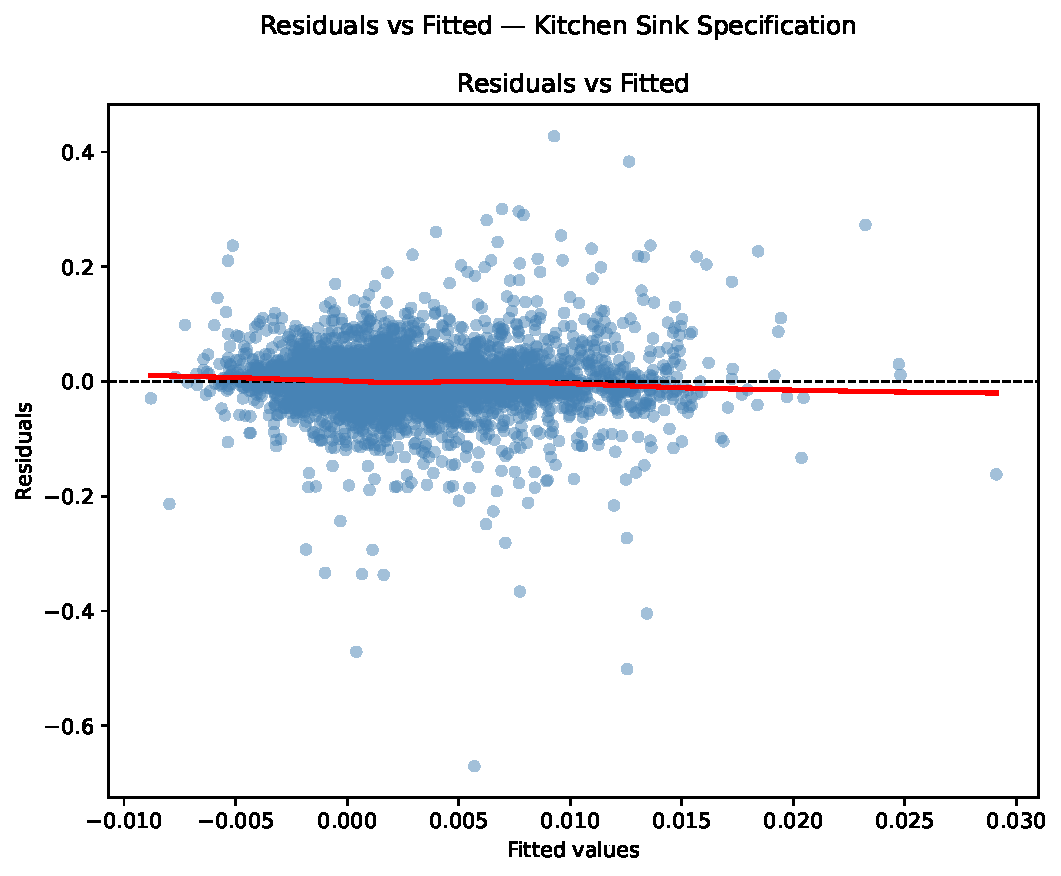
\includegraphics[width=0.85\textwidth]{../figures/btc_resid_vs_fitted.pdf}
\caption{Residuals vs Fitted Values --- Kitchen Sink Specification}
\label{fig:btc_resid}
\end{figure}

\begin{figure}[H]
\centering
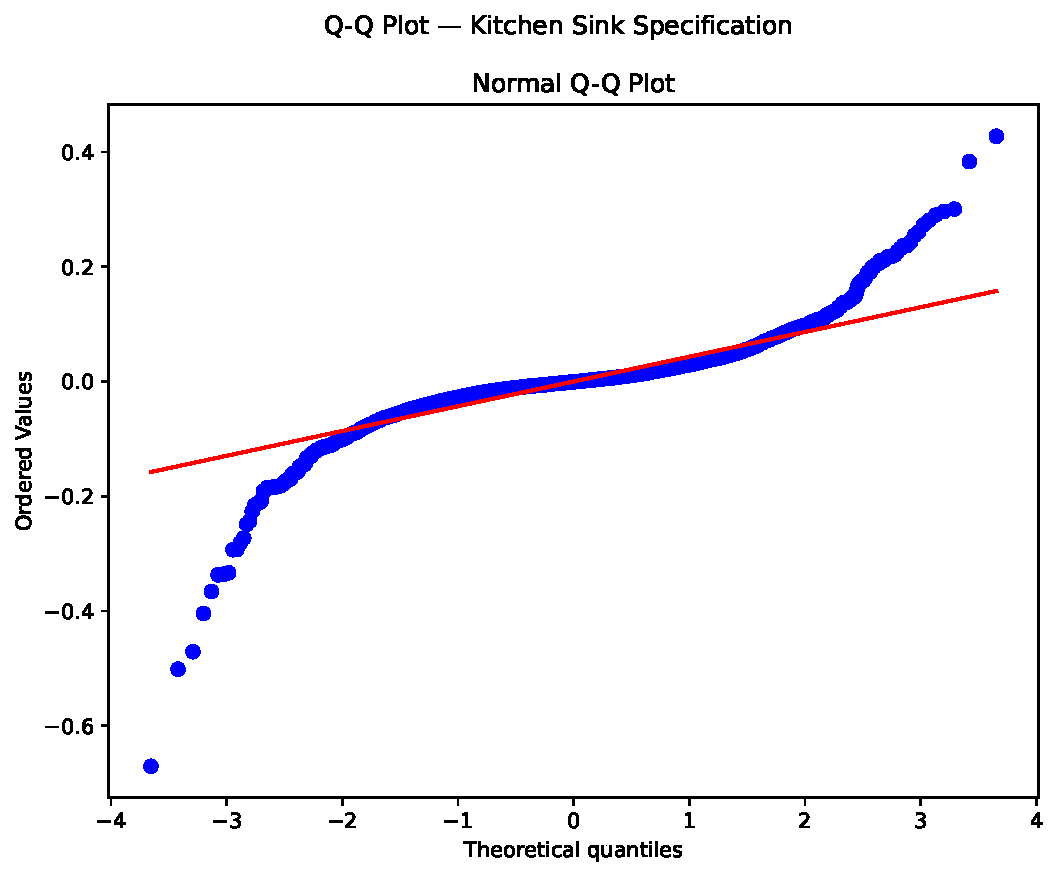
\includegraphics[width=0.65\textwidth]{../figures/btc_qq.pdf}
\caption{Q-Q Plot of Residuals}
\label{fig:btc_qq}
\end{figure}

The residual plots confirm the presence of heavy tails (clear departures
in the Q-Q plot) and some volatility clustering visible in the residuals
vs fitted plot. These features are typical of daily financial return data
and motivate our use of robust (HAC) standard errors.

\begin{figure}[H]
\centering
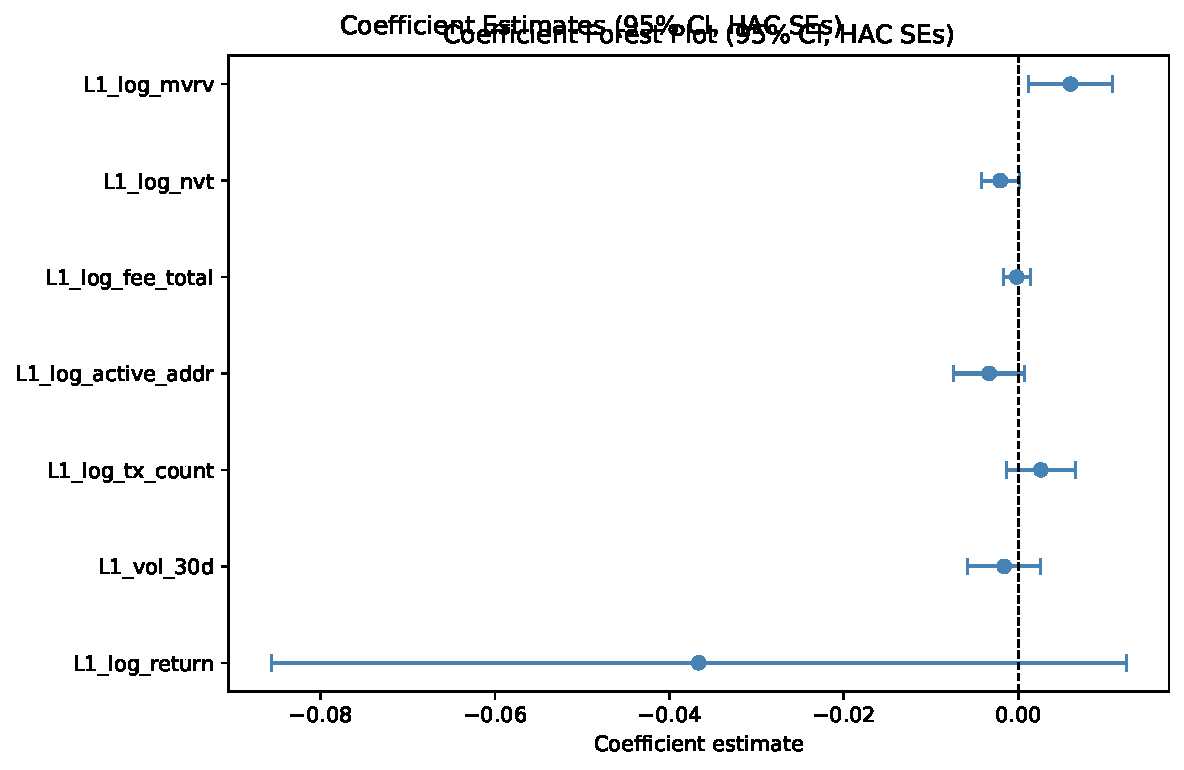
\includegraphics[width=0.75\textwidth]{../figures/btc_coef_forest.pdf}
\caption{Coefficient Estimates with 95\% Confidence Intervals (HAC SEs)}
\label{fig:btc_coef}
\end{figure}

\section{Conclusion}

Consistent with weak-form market efficiency, we find limited evidence that
lagged on-chain fundamentals predict short-horizon Bitcoin returns. The
MVRV ratio and certain network activity measures show marginal significance
in some specifications, but $R^2$ values remain very low across all models.
This is consistent with the broader empirical finance literature finding
that daily returns are largely unpredictable.

The diagnostic tests reveal substantial departures from classical assumptions---
heteroskedasticity, non-normality, and some residual autocorrelation---which
our HAC inference procedure addresses. Future work could explore longer
horizons, nonlinear specifications, or quantile regressions.

\begin{figure}[H]
\centering
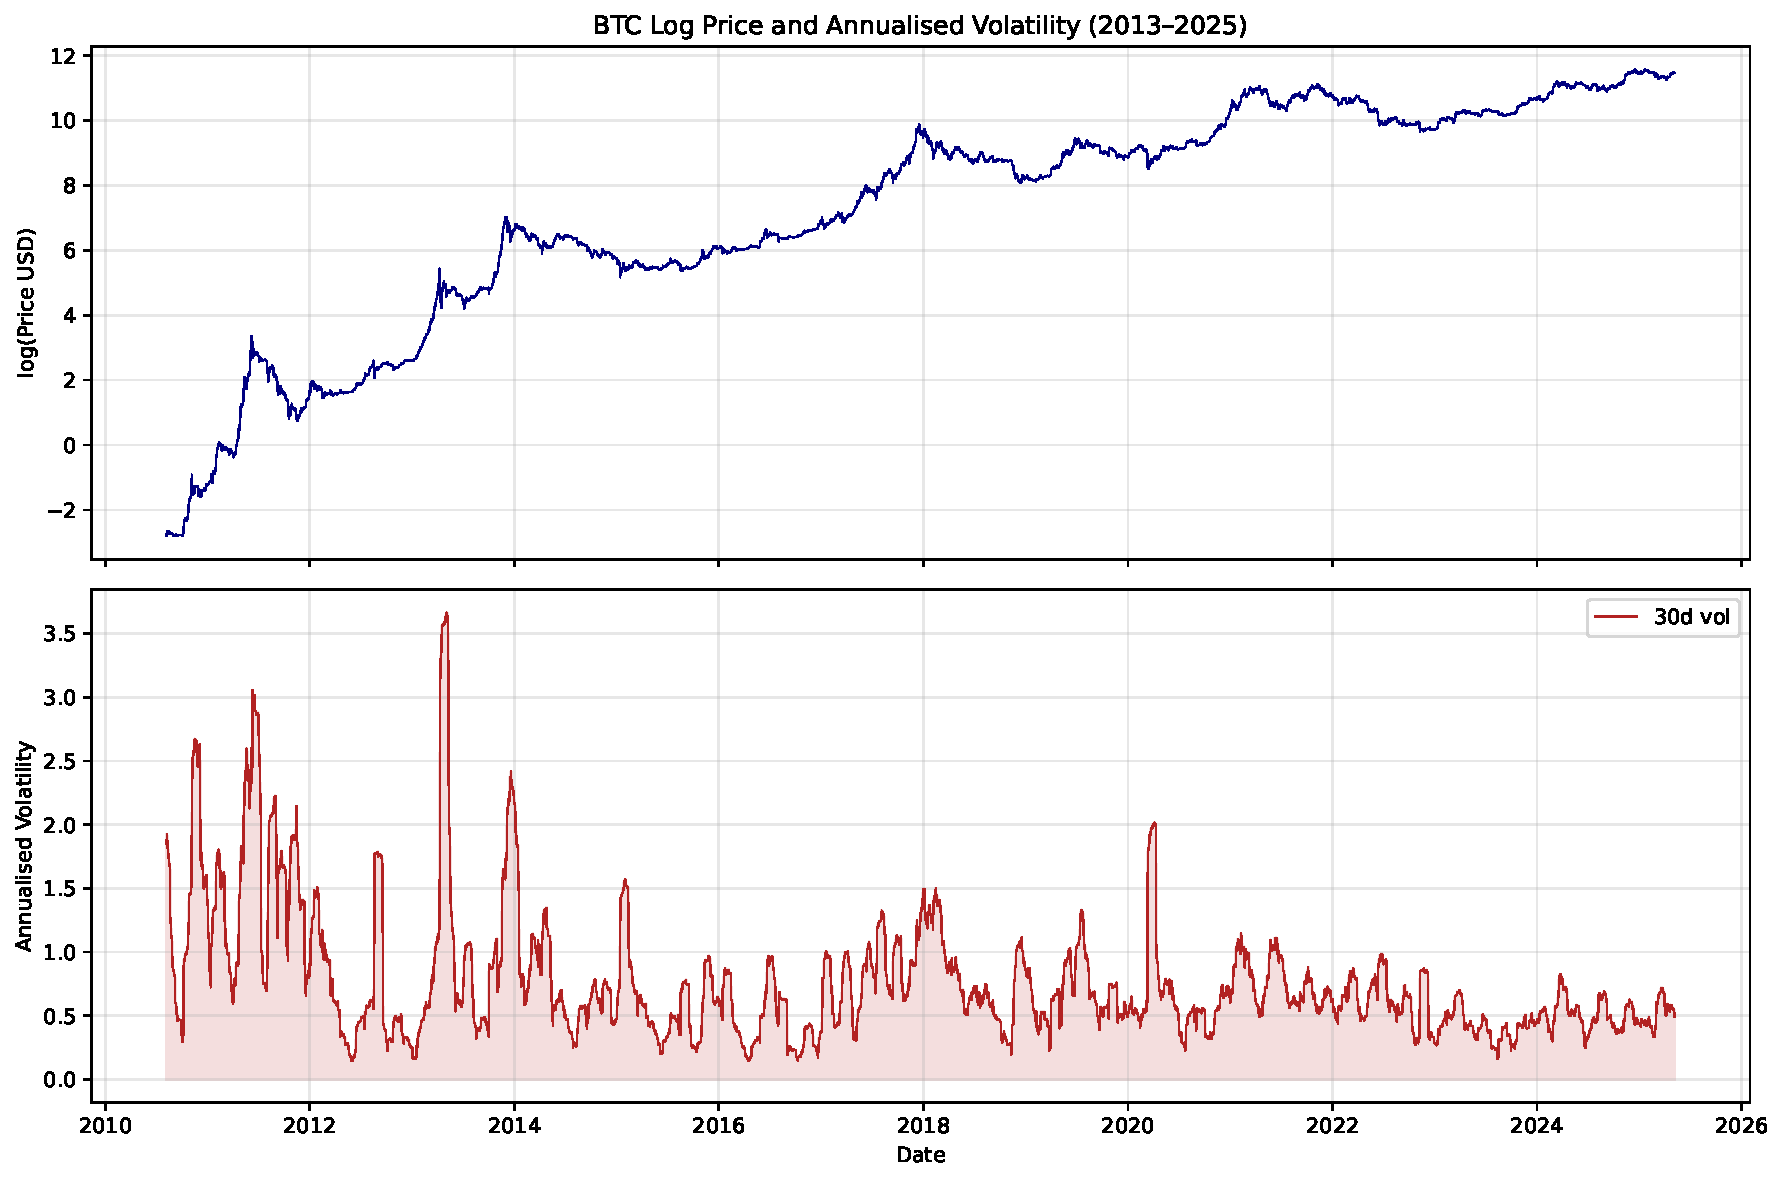
\includegraphics[width=\textwidth]{../figures/btc_price_vol_timeseries.pdf}
\caption{BTC Log Price and Annualised 30-Day Rolling Volatility}
\label{fig:btc_ts}
\end{figure}

\end{document}
